\documentclass[final,3p]{CSP}
\usepackage{amssymb}
\usepackage{changepage}
\usepackage{float}
\usepackage{hyperref}
\usepackage{url}
\usepackage{afterpage}
\usepackage{natbib}
\usepackage{setspace}
\usepackage{fancyhdr}
\pagestyle{fancy}
\fancyhf{}

\def\Student{Ashish Sehrawat}
\def\Title{THESIS PROJECT PROPOSAL}
\def\Prog{Doctorado en Ciencias (F\'{i}sica) }
\def\Dept{Departamento de Investigac\'{i}on en Fis\'{i}ca}
\def\Director{Dr. Jos\'{e} Feliciano Ben\'{i}tez Rubio}
\def\ProjectTitle{ Measurement of ... }
\def\ResearchLine{Astrof\'{i}sica, Cosmolog\'{i}a y F\'{i}sica de Part\'{i}culas}


\newcommand{\SubItem}[1]{
    {\setlength\itemindent{15pt} \item[-] #1}
}


%%header and footer
\lhead{\Student}
\rhead{\Title}
\lfoot{\Dept}
\rfoot{Page \thepage}
\setlength{\headsep}{0.2in}
\renewcommand{\footrulewidth}{0.4pt}% default is 0pt


\begin{document}

%%%%Title Page
\begin{titlepage}
  \centering
  \hspace{0pt}
  \vfill
        {\scshape\Large \Title \par}

	\vspace{2cm}
        \begin{adjustwidth}{2cm}{2cm}{
            TITLE:\par
            {\large \ProjectTitle \par}
          }
        \end{adjustwidth}

	\vspace{0.5cm}
        \begin{adjustwidth}{2cm}{2cm}{
            RESEARCH LINE: \par
            \ResearchLine \par}
        \end{adjustwidth}

        
        \vspace{4cm}
        {\underline{\hspace{8cm}}\par}
	{\scshape\large \Student \par}
        {Student\par}

        \vspace{1cm}
        {\underline{\hspace{8cm}}\par}
	{\Director \par}
        {Director\par}

        \vspace{1cm}
        {\Prog \par}
        {\Dept \par}
        {Universidad de Sonora \par}

        \vspace{4cm}
	{\today}

\hspace{0pt}
\vfill

\end{titlepage}


%%%%% white page for print out
\shipout\null


%%%% Abstract Page
\newpage
\hspace{2pt}
\vfill

\begin{adjustwidth}{1cm}{1cm}

  \begin{center}
    {\Large \ProjectTitle \par}
    \vspace{1cm}
    {\itshape\textbf{Abstract}\par}
  \end{center}
  
  \vspace{1 cm}
 
  
  \onehalfspacing
  This research project proposes ...

\end{adjustwidth}

\hspace{2pt}
\vfill

%%%%%% Begin the body
\newpage
\section{BACKGROUND}


\onehalfspacing The standard model (SM) of particle physics is so far the best theoretical model to describe the interaction of elementary 
particles using three of the four fundamental forces of nature which are electromagnetic force, strong nuclear force and the 
weak nuclear force. Gravitational force is neglected as the strength of this force is very weak at the scales over which 
elementary particle interact with each other. The standard model (SM) of particle physics is divided into two categories, 
bosonic sector and fermionic sector. Bosonic sector contain particles called bosons which mediate the fundamental forces of 
nature and the fermionic sector contain particles called fermions which make up all the matter in our universe. SM has three 
generations of matter (fermions) particles. The first generation of fermions consists of up (u) quark, down (d) quark, electron 
and electron neutrino, second generation consist of charm (c) quark, strange (s) quark, muon and muon neutrino and the third 
generation of matter particles has top (t) quark, bottom (b) quark, tau and tau neutrino. The bosonic sector consist of gauge 
bosons like gluon, photon, $W^{\pm}$, $Z^0$ which mediate strong nuclear force, electromagnetic force and weak nuclear force respectively. There is one more particle in the standard model called the Higgs Boson which gives mass to SM particles via electroweak symmetry breaking mechanism \cite{Chatrchyan:2012xdj}. All the standard model particles are shown in Figure 1. Higgs boson can be produced at the particle colliders like the Large Hadron Collider (LHC) in Geneva, Switzerland.



The Standard Model (SM) of particle physics has successfully described most of the experimental data till now but a very large 
number of free-parameters and the fine tuning related to these parameters suggest new physics beyond SM as mentioned below.
\begin{itemize}
\item{Fine structure constant $\alpha$},
\item{Weinberg angle or the weak mixing angle $\theta_W$},
\item{The coupling constant of strong interaction $\alpha_s$},
\item{Electroweak symmetry breaking energy scale v},
\item{ Higgs potential self coupling $\lambda$ or the Higgs mass $m_H$},
\item{Three weak mixing angles and the CP-violating phase $\delta$ of the CKM matrix which tells us how quarks of different flavor mix with each other},
\item{Nine yukawa couplings $y_i$ (i = 1 to 9) which determine the mass of nine charged fermions}.
\end{itemize}


Until the 90's the existence of almost all the particles of the SM were confirmed except the top quark and the Higgs boson. 
These had eluded previous experiments due to difficulties in the production or reconstruction of its decays. The top quark was 
discovered in 1995 in the Tevatron collider of the Fermilab laboratory, this proton collider operated with a center of mass 
energy of 1.8 TeV untill 2010. The LHC collider at the CERN laboratory in Geneva, Switzerland, began its operations in 2010 
colliding protons at 7 TeV increasing the colliding energies to 8 and 13 TeV in the subsequent years. The Compact Muon Solenoid (CMS) is based on the Large Hadron Collider (LHC). It is designed to detect particles known as muons very accurately. The CMS detector has the form of a cylindrical onion, with several concentric layers of components. Needed a powerful magnet to bend charged particles as they move away from the point of collision to identify the charge of the particles to bend them in opposite directions and measure momentum. A silicon tracker, made of about 75 
million electronic sensors arranged in concentric layers, identifies the tracks taken by these charged particles bent with very high precision \cite{Chatrchyan:2008aa}. The muons are detected by special subdetectors placed outside to detect them once they have crossed the solenoid as shown in Figure~\ref{figure5}. In 2012, the ATLAS and CMS collaborations, with detectors at two points where the protons collide in the LHC, announced the discovery of a new boson with a mass of 125 GeV. So far, all measurements of the properties of this boson are consistent with those of the Higgs boson of the Standard Model (SM).


LHC during the first run in 2011 and 2012 reached a peak instantaneous luminosity of 7.7 $\times$ $10^{33}$ $cm^{-2}s^{-1}$ which was more than 75$\%$ of its design luminosity and delivered an integrated luminosity of about 25 $fb^{-1}$ to each ATLAS and CMS.
 The LHC will deliver about 300 $fb^{-1}$ by 2024 \cite{collaborations2019report}.
The goal of subsequently run of LHC has been to obtain datasets at higher values of luminosities for precision measurements of the properties of Higgs boson, in order to test the Standard Model pattern of couplings to elementary particles.
In order to minimize the machine downtimes and maximize the productive use of the LHC for physics, the replacement of the inner triplet magnets (the one responsible to squeeze the beam at collision) and  of  all  hardware  changes  needed  to  enable  an  ambitious  luminosity  upgrade  will  take  place in parallel during one shutdown, at around 2023-25 (LS3), with some of the modification anticipated in 2019-2020 (LS2).
This new phase of the LHC life has been named as High Luminosity LHC (HL-LHC) and has the scope of attaining the astonishing threshold of 3000 $fb^{-1}$ by the year 2036 as shown in Figure~\ref{figure6}.
Figure~\ref{figureKappas} shows a summary of the current measurements of the Higgs coupling parameters with the LHC Run 1 dataset (2011,2012)  using ggF, VBF, VH, and ${t\bar{t}H}$ production modes \cite{Tanabashi:2018oca}.





\begin{figure}[H]
        \centering
        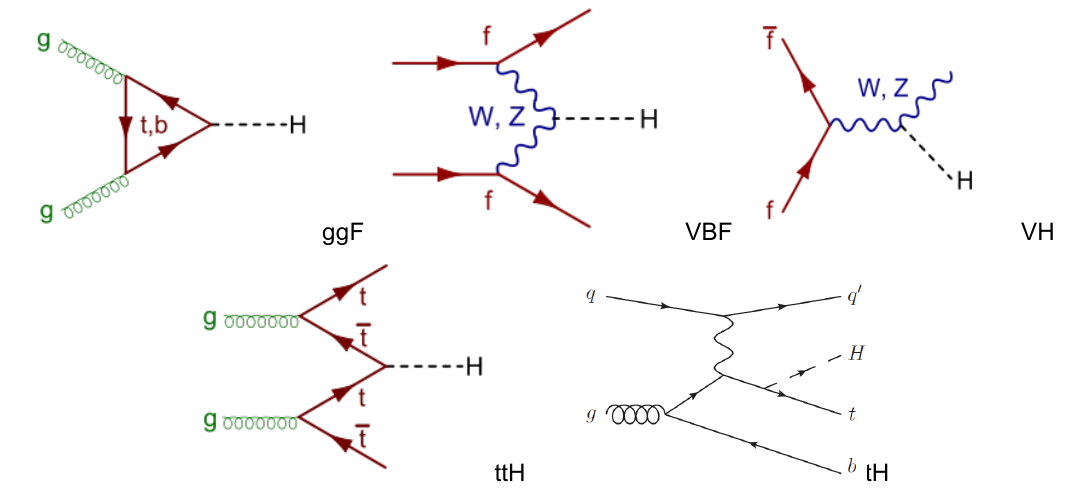
\includegraphics[width=\columnwidth]{./pg.png}
        \caption{Important production processes of Standard model Higgs boson ggF, VBF, VH, ttH and tH in proton collisions.}
        \label{figure 2}
\end{figure}


%\begin{figure}[H]
%  \centering
%   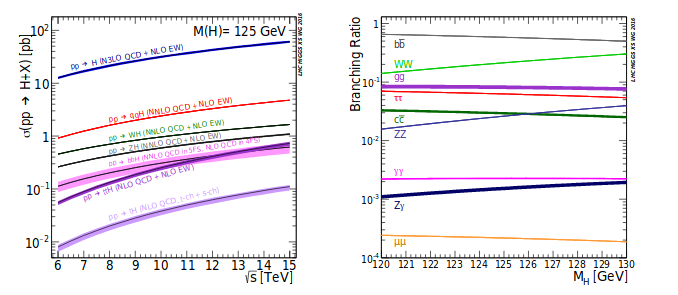
\includegraphics[width=\columnwidth]{./cd2.png}
%  \caption{Standard model Higgs boson production cross section with center of mass energy and branching ratios for various decay channels.}
%   \label{figure 3}
%\end{figure}

\begin{figure}[H]
  \centering
  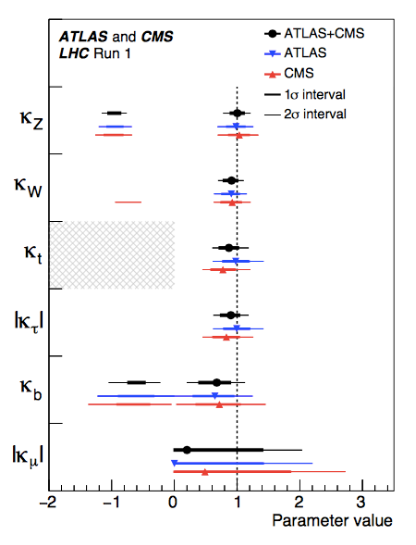
\includegraphics[scale=0.4]{./couplings.png}
  \caption{ATLAS-CMS combined measurements of coupling strength modifiers \cite{Tanabashi:2018oca}.}
  \label{figureKappas}
\end{figure}


\begin{figure}[H]
  \centering
  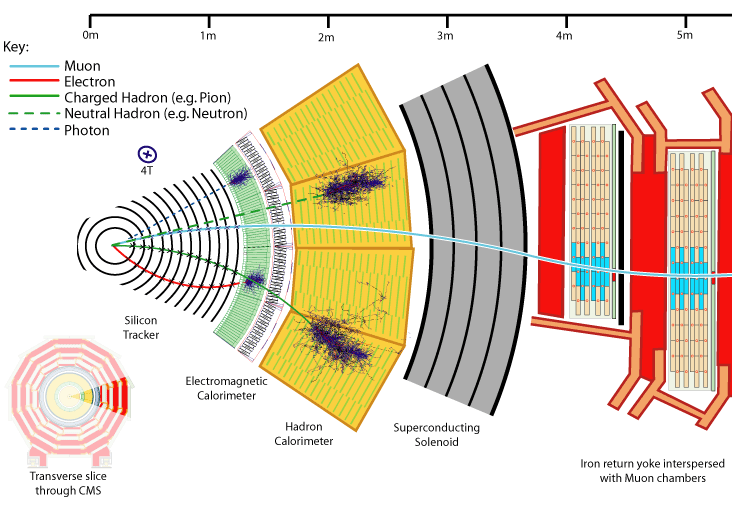
\includegraphics[width=0.6\columnwidth]{./cms12.png}
  \caption{Transverse view of the CMS detector showing the silicon tracker, electromagnetic calorimeter, hadron calorimeter, superconducting solenoid and muon chambers \cite{Chatrchyan:2008aa}.}
  \label{figure5}
\end{figure}

\begin{figure}[H]
  \centering
  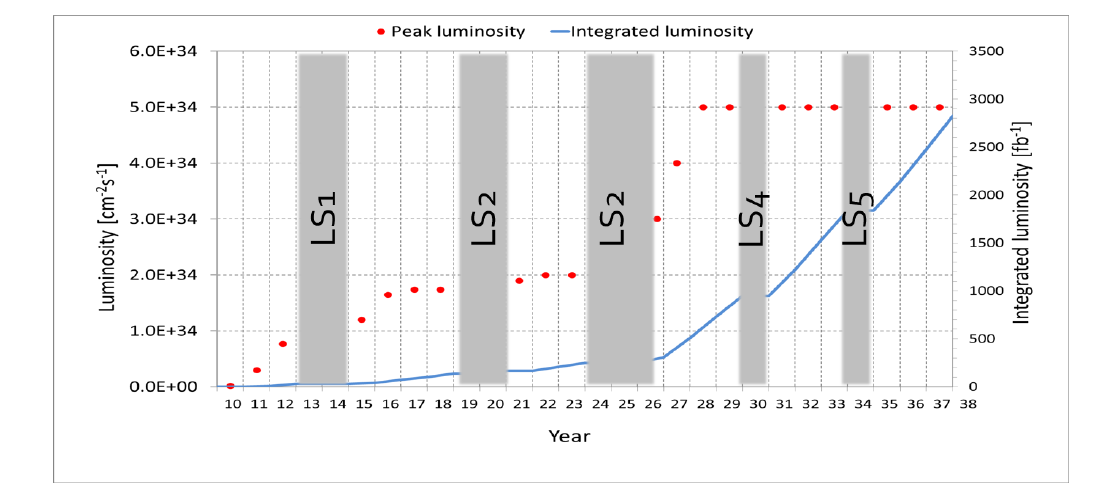
\includegraphics[width=0.9\columnwidth]{./lum6.png}
  \caption{Projected performance of the LHC until 2038, which shows the preliminary dates for prolonged stops (LS) of the LHC and luminosities. Points show instantaneous luminosity while the line shows luminosity accumulated \cite{collaborations2019report}.}
  \label{figure6}
\end{figure}


  
\newpage
\section{PROPOSAL}

\onehalfspacing
In this project, it is proposed to


\section{GENERAL OBJECTIVE}

%- motivation, tH production crossection, sign of $k_t$, search for BSM, ..

\onehalfspacing
There is currently a great enigma in physics since we know that ordinary matter comprises only $5\%$ of the universe, another $27\%$ includes Dark matter and the rest $68\%$ is Dark energy.


\section{HYPOTHESIS}
%%  - what we expect to find

\onehalfspacing

%\newpage
\section{SPECIFIC OBJECTIVES}

\onehalfspacing

In order to complete a journal publication ...

\begin{itemize}
\item Simulation..
\end{itemize}

Finally, the results of this project will be presented at national or international conferences and a publication in a scientific journal will be accomplished.


\section{METHODOLOGY}

\onehalfspacing
The methods for ...


\textsc{Root} is a \textsc{c++} based software that allows visualization of event distributions and variable correlations.


\section{EXPECTED RESULTS}
%- a limit, also predictions for future runs

\onehalfspacing The results from this project include the following items:
\begin{itemize}
\item The student will become part of an international collaboration.
\item A leading contribution ....  resulting in a publication in a scientific journal.
\item Participation in the CMS detector Phase II upgrade through development and possible installation of particle detectors possibly resulting in a technical report.
\item A presentation of a poster or a talk in one of the national conferences of the Division of Paticles and Fields of the Mexican Society of Physics or a presentation of a poster or a talk in an international physics conference.
\item An academic stay at a scientific center like CERN or Fermilab.
\end{itemize}



\section{CALENDAR OF ACTIVITIES}
\onehalfspacing
\begin{itemize}

\item {\bf Semester 1 (2019-2)}:
  \SubItem{ Readings on Standard Model theory}
  \SubItem{ Basic Linux computing skills (\textsc{Bash, Emacs, Root})}
  \SubItem{ Initial planning of the analysis strategy}

\item {\bf Semester 2 (2020-1)}:
  \SubItem{ Course I on particle physics and/or particle detection}
  \SubItem{ Basic Linux computing skills (\textsc{Bash, Emacs, Root})}
  \SubItem{ Readings on SM and tH literature}
  \SubItem{ Computing accounts at CERN and Fermilab}
  \SubItem{ CMS service work for authorship}
  \SubItem{ Possible summer stay at CERN or Fermilab}

\item {\bf Semester 3 (2020-2)}:
  \SubItem{ Course II on particle physics and/or particle detection.}
  \SubItem{ CMS service work for authorship}

\item {\bf Semester 4 (2021-1)}:
  \SubItem{ CMS service work for authorship}

\item {\bf Semester 5 (2021-2)}:
  \SubItem{ Presentation of poster or talk at national or international conference}

\item {\bf Semester 6 (2022-1)}:
  \SubItem{ Review process of the results within the CMS collaboration}
  \SubItem{ Presentation of poster or talk at national or international conference}
  \SubItem{ Writing of the paper publication}
  \SubItem{ Writing of the thesis}
\end{itemize}



\cleardoublepage
\onehalfspacing
\bibliographystyle{unsrt}
\bibliography{paper}

\end{document}

